% 2018 江苏卷第15题：平行六面体 ABCD-A1B1C1D1
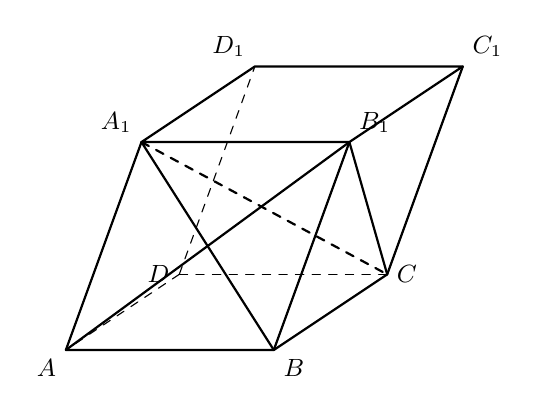
\begin{tikzpicture}[font=\small, line cap=round, line join=round, >=stealth, scale=1.2]
  % 顶点坐标
  \coordinate (A) at (0, 0);
  \coordinate (B) at (2.2, 0);
  \coordinate (C) at (3.4, 0.8);
  \coordinate (D) at (1.2, 0.8);
  \coordinate (A1) at (0.8, 2.2);
  \coordinate (B1) at (3.0, 2.2);
  \coordinate (C1) at (4.2, 3.0);
  \coordinate (D1) at (2.0, 3.0);

  % 隐藏棱（虚线）
  \draw[dashed, thin] (D) -- (A);
  \draw[dashed, thin] (D) -- (C);
  \draw[dashed, thin] (D) -- (D1);
  \draw[dashed, thick] (A1) -- (C);

  % 可见棱（实线）
  \draw[thick] (A) -- (B) -- (C);
  \draw[thick] (A1) -- (B1) -- (C1) -- (D1) -- cycle;
  \draw[thick] (A) -- (A1);
  \draw[thick] (B) -- (B1);
  \draw[thick] (C) -- (C1);

  % 辅助线/对角线
  \draw[thick] (A) -- (B1);
  \draw[thick] (A1) -- (B);
  \draw[thick] (B1) -- (C);

  % 顶点标签
  \node[below left] at (A) {$A$};
  \node[below right] at (B) {$B$};
  \node[right] at (C) {$C$};
  \node[left] at (D) {$D$};
  \node[above left] at (A1) {$A_1$};
  \node[above right] at (B1) {$B_1$};
  \node[above right] at (C1) {$C_1$};
  \node[above left] at (D1) {$D_1$};
\end{tikzpicture}
